\chapter{Задача конвертации данных и графических файлов DXF. Анализ текущего состояния проблемы исследования}
\label{cha:aktuell}

В данном разделе описаны экономические аспекты проекта по созданию ПО <<Primiview>> для обработки геометрической информации 2D-объектов специального типа.

\section{Графические форматы файлов в САПР}
Конвертер в TXT по типу DXF применяется для контроля содержания необходимых (поддерживаемых) примитивов (объектов) в DXF-файле. Также, с помощью данного формата может производится расчёт длины траектории  контура детали (обычно, в поперечном её сечении). Это может быть полезно при применении ПО в области лазерной резки с помощью станков с ЧПУ, а, в частности, в ПО <<Сириус>>.

Конвертер из DXF в TXT в формате координат и радиуса применяется для автоматизированного технологического проектирования, для формирования УП. Получаемая в результате работы ПО информация о примитивах изображения контура детали используется для непосредственного составления УП, так как каждая последующая точка имеет не только плоские координаты, но и способ достижения этой точки (тип примитива: отрезок, если радиус равен нулю; дуга, если радиус ненулевой).

Конвертер в SVG-формат полезен для последующего формирования других типов файлов (например, DBS), а также, для компактного по объёму файла векторного представления контура детали. ИВЗУАЛИЗАЦИЯ. ПОДробно о svg - литературный обзор. Внутренняя репрезентация (ezdxf)

Конвертер в JSON удобен для хранения информации об объектах контура детали. В этом формате работает и другое ПО разрабатываемой САПР для формирования УП для станков с ЧПУ.

В целом, разрабатываемый набор конвертеров (модуль экспорта) представляет собой цельный ПП, сочетающий в себе набор необходимых разработчику УП начальных функций для автоматизированного технологического проектирования. Это ПО может быть интегрировано в разные ПП, так как по сути универсально в своём применении (используется в области 2D-резки, токарной обработке).


\subsection{Формат DXF}

\paragraph{Краткая характеристика}

\begin{longtable}{p{110pt} p{340pt}}
%	\caption{}
	\label{tab:dxf}
	\centering
	\textbf{Название}:&AutoCAD DXF\\
	\textbf{Также известен как}:&AutoCAD Drawind Interchange Format, DXF, .DXB, .SLD, .ADI\\
	\textbf{Тип данных}:&Векторный\\
	\textbf{Сжатие}:&нет\\
	\textbf{Максимальный размер изображения}:&неограниченный\\
	\textbf{Несколько изображений в одном файле}:&нет\\
	\textbf{Разработчик}:&Autodesk\\
	\textbf{Поддерживающ. приложения}:&AutoCAD, различные САПР, CorelDraw, др.\\
	\textbf{Использование}:&Хранение и обмен САПР-(проектировочными) и векторными данными\\
	\textbf{Комментарии}:&Сложный формат, в основном, потому что может содержать в себе много различных типов данных. Формат разработан и поддерживается компанией Autodesk с целью применения в CAD-системе AutoCAD. Самая распространённая форма DXF --- 7-битный текст, однако существует, также, два схожих двоичных формата, один из которых представляется в виде расширения DXF, а другой --- DXB.\\
\end{longtable}

\paragraph{Обзор}

Форматы AutoCAD DXF (Drawing Interchange Format) и AutoCAD DXB (Drawing Interchange Binary) связаны с CAD-системой AutoCAD, созданной и поддерживаемой Autodesk. DXB — это упрощенная двоичная версия файла DXF. Другими форматами файлов, связанными с AutoCAD, являются форматы слайдов (.SLD) и графиков (.ADI).

Несмотря на то, что DXF был разработан для представления данных в САПР, он используется многими другими программами как формат обмена многими различными типами данных, чаще всего векторно-ориентированной информацией, а также текстом и 3D-полигонами. Как формат САПР, он также может выражать общие концепции черчения, такие как ассоциативные размеры.

Почти любой тип данных может быть каким-либо образом представлен в DXF. Например, программа для рисования CorelDraw! экспортирует контуры чертежа с объектом AutoCAD POLYLINE, в то время как 3D-программа может экспортировать только объекты 3DFACE, представляющие трёх- и четырёхсторонние многоугольники. DXF, также, позволяет создавать множество способов делать почти одно и то же, например, описывать объекты как отдельные редактируемые группы. Одна программа может размещать объекты на разных слоях рисунка, в то время как другая может использовать разные цвета пера, а третья может использовать именованные «блоки» для группировки данных.

Хоть DXF и широко используется для обмена простыми линейными данными, разработчик приложений, желающий поддерживать в них DXF, должен учитывать, что AutoCAD может хранить эти многочисленные типы данных различными способами.

Иногда правильная интерпретация файла DXF может быть очень сложной. Предполагаемый внешний вид линий и областей может зависеть от многих, казалось бы, непонятных настроек в заголовке DXF-файла. Поскольку файлы DXF очень сложно правильно интерпретировать, многие разработчики приложений решают экспортировать только DXF.

Даже среди программ, заявляющих об импорте DXF, можно обнаружить, что они поддерживают лишь часть всего, что возможно в DXF. Если есть необходимость создать свои собственные файлы DXF для передачи данных в программу, которая утверждает, что импортирует DXF, нужно убедиться, что известно, какие представления она понимает.

С каждой новой версией AutoCAD, DXF изменяется. AutoCAD версии 13 расширил формат DXF во многих отношениях, чтобы представить специализированные данные нового механизма геометрии. Эти дополнения хранят информацию о сложных поверхностях и твёрдых телах для геометрического механизма ACIS компании Spatial Technology, который теперь является частью AutoCAD. Не вся эта информация была задокументирована и должна быть пропущена любым читателем DXF. В версии 13 собственный допуск AutoCAD для числовых файлов DXF также изменился, поскольку он расширил шаг аудита, который проверяет достоверность импортируемых файлов DXF.

Очевидно, что формат файла DXF довольно сложный и тонкий. Далее приведена базовая структура любого файла DXF.

\paragraph{Организация файла}

Файл DXF состоит из семи разделов: заголовка, таблиц, блоков, классов, объектов, сущностей и маркера конца файла.

\begin{itemize}
	\item Раздел HEADER содержит переменные, представляющие состояние внутренних настроек AutoCAD. Например, для переменной версии AutoCAD «\$ACADVER» установлено значение «AC1012» в файле DXF, сохраненном AutoCAD версии 13. Другие переменные задают единицы измерения углов, значения по умолчанию для снятия фаски, смещения, масштабирования и т. д.
	\item Раздел TABLES содержит несколько массивов информации, используемой в остальной части чертежа, например список типов линий, имён слоев, шрифтов и предустановленных видов чертежа.
	\item Раздел BLOCKS содержит предопределенные элементы чертежа, которые могут присутствовать на чертеже. Например, блок может определять стандартную канавку, которая размещается на каждой секции вала определённого диаметра на чертеже. На определения блоков ссылаются в разделе ENTITIES с помощью команды INSERT.
	\item Разделы CLASSES и OBJECTS были представлены начиная с AutoCAD версии 13. Раздел CLASSES содержит описание любых определяемых приложением классов объектов, которые могут быть реализованы в разделах BLOCKS или ENTITIES.
	\item Раздел OBJECTS содержит неграфические части чертежа. Все сущности, которые не являются частью сущностей или таблиц символов, являются «объектами». Например, здесь хранятся словари AutoCAD.
	\item Раздел ENTITIES содержит фактические данные объекта чертежа. Сюда могут входить необработанные данные, такие как объекты LINE и ARC, а также команды INSERT, которые помещают предопределенное определение блока в определенную позицию на чертеже.
	\item Конец данных DXF отмечается директивой EOF в последней строке файла.
\end{itemize}

\paragraph{Детали файла}
Файл DXF состоит из пар групповых кодов и связанных значений. Каждое из них находится в отдельной строке текстового файла. Целочисленный групповой код указывает тип значения, за которым следует. Групповые коды встречаются в диапазонах. Например, за групповыми кодами от 0 до 9 следуют строки, и каждый отдельный групповой код используется в определенных случаях. Групповой код 0 указывает на начало объекта, таблицы или индикатора конца файла. Код 1 указывает основное текстовое значение объекта. Код группы 2 используется для имён, таких как имена разделов, блоков, имен таблиц и т. д. Код 9 вводит имя переменной раздела заголовка. Например, в начале каждого файла DXF код группы 0 предшествует команде SECTION, за которой следует код группы 2 со строкой, указывающей тип раздела, например HEADER:

\begin{lstlisting}[label=list:dxfheader]
0
SECTION
2
HEADER
9
$ACADVER
1
AC1012
\end{lstlisting}

Диапазоны групповых кодов указывают тип данных, которым следует следовать. Групповые коды от 10 до 59 используются для значений с плавающей точкой, таких как координаты точек. Коды с 60 по 79 хранят целочисленные значения. Например, для сохранения местоположения 2D-точки сначала используется групповой код 10 для значения X, затем код 20 используется для значения Y. Если объект имеет вторичное значение координаты, он также будет использовать групповые коды 11 и 21. Вот минимальный, но полный файл DXF, который описывает линию от точки (1,2) до (3,4) в плоском пространстве:

\begin{lstlisting}[label=list:dxflinefull]
0
SECTION
2
ENTITIES
999
This is just a line
0
LINE
8
0
10
1.0
20
2.0
11
3.0 21
4.0 0
ENDSEC
0
EOF
\end{lstlisting}

Код группы 999 предшествует комментарию. Эта строка будет помещена на слой 0, на что указывает групповой код 8. Этот минимальный файл является примером файла «только объекты», который будет принят практически любой программой, которая утверждает, что импортирует DXF.

Поскольку AutoCAD расширяется с каждой новой версией, добавляются новые групповые коды. При написании программы, которая читает файлы DXF, можно обеспечить совместимость в будущем, игнорируя неопределенные пары кода группы и значения.
Одним любопытным аспектом DXF является то, что он не содержит цветовой палитры, однако большинству объектов в файле DXF можно присвоить отдельное значение цвета с групповым кодом 62. Каждому объекту чертежа может быть присвоен номер от 1 до 255, известный как AutoCAD Color Index, или ACI, также описанный в более ранней документации как «номер пера». Это отражает происхождение AutoCAD как пакета САПР, в котором чертежи обычно печатались на перьевом плоттере с несколькими чернильными перьями, но без стандартного соответствия фактическим значениям RGB или даже цветам линий на экране. AutoCAD теперь устанавливает цвет RGB по умолчанию для каждого ACI, когда он появляется на экране, но они не сохраняются в файле DXF \cite{murray1996encyclopedia}.

\subsection{Формат SVG}
\paragraph{Краткая характеристика}

\begin{longtable}{p{110pt} p{340pt}}
	%	\caption{}
	\label{tab:svg}
	\centering
	\textbf{Название}:&image/svg+xml\\
	\textbf{Также известен как}:&SVG, SVGZ (изображения, сд=жатые с помощью gzip)\\
	\textbf{Тип данных}:&Векторный/растровый\\
	\textbf{Сжатие}:&SVGZ\\
	\textbf{Максимальный размер изображения}:&неограниченный\\
	\textbf{Несколько изображений в одном файле}:&нет\\
	\textbf{Разработчик}:&World Wide Web Consortium (SVG Working Group)\\
	\textbf{Поддерживающ. приложения}:&браузеры, редакторы изображений, инструменты и библиотеки\\
	\textbf{Использование}:&Доступный обзор и обмен векторными изображениями, построение графиков, сложные элементы пользовательского интерфейса, логотипы, простые игры\\
	\textbf{Комментарии}:&Язык для описания двумерной графики в XML, созданный Консорциумом Всемирной паутины (W3C). Поддерживает как неподвижную, так и анимированную интерактивную графику — или, в иных терминах, декларативную и скриптовую. Не поддерживает описания трёхмерных объектов.\\
\end{longtable}

\paragraph{Обзор}

SVG - это язык для описания двумерной графики в XML [XML10, XML11]. SVG позволяет создавать графические объекты трех типов: векторные графические фигуры (например, контуры, состоящие из прямых линий и кривых), мультимедиа (растровые изображения, видео и аудио) и текст.

Документы SVG могут быть интерактивными и динамическими. Анимации могут быть определены и запущены либо декларативно (то есть путем встраивания анимационных элементов SVG в содержимое SVG), либо с помощью сценариев.

Достоинством формата SVG можно назвать, среди прочего, его представление в текстовом формате, то есть файлы SVG можно читать и редактировать при помощи обычных текстовых редакторов. При просмотре документов, содержащих SVG-графику, имеется доступ к просмотру кода просматриваемого файла и возможность сохранения всего документа. Кроме того, SVG-файлы обычно получаются меньше по размеру, чем сравнимые по качеству изображения в форматах JPEG (Joint Photographic Experts Group) или GIF (Graphics Interchange Format ), а также хорошо поддаются сжатию.

Масштабируемость изображения в формате SVG подразумевает возомжность увеличить любую часть изображения SVG без потери качества.

Широко доступно использование растровой графики в SVG-документах позволяет вставлять элементы с изображениями в форматах PNG, GIF или JPG.

Текст в графике SVG является текстом, а не изображением, поэтому его можно выделять и копировать, он индексируется поисковыми машинами, для этого не требуется создавать дополнительные метафайлы для поисковых роботов.

Анимация реализована в SVG с помощью языка SMIL (Synchronized Multimedia Integration Language), разработанного также консорциумом W3C. Поддерживаются скриптовые языки на основе спецификации ECMAScript. SVG-элементами можно управлять с помощью JavaScript. Применение скриптов и анимации в SVG позволяет создавать динамичную и интерактивную графику. В SVG обеспечивается событийная модель, отслеживаются события (загрузка страницы, изменение её параметров, события мыши, клавиатуры и др.). Анимация может запускаться по определённому событию (например «onmouseover» или «onclick»), что придаёт графике интерактивность. У каждого элемента есть свои собственные события, к которым можно привязывать отдельные скрипты.

SVG — открытый стандарт. В отличие от некоторых других форматов, SVG не является чьей-либо собственностью.

SVG-документы легко интегрируются с HTML-(HyperText Markup Language — «язык гипертекстовой разметки») и XHTML-документами. Внешние SVG подключаются через тег <object>, значение атрибута data — имя файла с расширением «.svg», содержащего разметку SVG, и имеющего MIME-тип image/svg+xml. Атрибуты width и height определяют размеры области SVG по горизонтали и по вертикали. Элементы SVG совместимы с HTML и DHTML (Dynamic HTML).

SVG предоставляет все преимущества XML:
\begin{itemize}
	\item Возможность работы в различных средах;
	\item Интернационализация (поддержка Юникода);
	\item Широкая доступность для различных приложений;
	\item Лёгкая модификация через стандартные API — например, DOM. SVG поддерживает стандартизированную W3C объектную модель документа DOM, обеспечивая доступ к любому элементу, что даёт широкие возможности по динамическому изменению элементов, их атрибутов и событий.;
	\item Лёгкое преобразование таблицами стилей XSLT. Как любой основанный на XML формат, SVG даёт возможность использовать для его обработки таблицы трансформации (XSLT). Преобразуя XML-данные в SVG с помощью простого XSL, можно легко получить графическое представление любых данных, например визуализировать химические молекулы, описанных на языке CML.
\end{itemize}

\paragraph{Организация файла}

Фрагмент документа SVG состоит из любого количества Элементы SVG содержится в "svg" элемент, включающий "svg" элемент.

Фрагмент документа SVG может варьироваться от пустого фрагмента (т. Е. без содержимого внутри "svg" элемент), для очень простого Фрагмент документа SVG содержащая один SVG графический элемент такая как "прямоугольник" для сложной, глубоко вложенной коллекции элементы контейнера и графические элементы.

Фрагмент документа SVG может существовать сама по себе как автономный файл или ресурс, в этом случае Фрагмент документа SVG является документом SVG, или он может быть встроен в качестве фрагмента в родительский XML-документ.

В следующем примере показано простое содержимое SVG, встроенное в виде фрагмента в родительский XML-документ. Обратите внимание на использование пространств имен XML, чтобы указать, что "svg" и "эллипс" элементы принадлежат пространству имен SVG:
\begin{lstlisting}[language=XML,label=list:xml]
<?xml version="1.0"?>
<parent xmlns="http://example.org"
  xmlns:svg="http://www.w3.org/2000/svg">
  <!-- parent contents here -->
  <svg:svg width="4cm" height="8cm" version="1.2" baseProfile="tiny" viewBox="0 0 100 100">
  <svg:ellipse cx="50" cy="50" rx="40" ry="20" />
  </svg:svg>
  <!-- ... -->
</parent>
\end{lstlisting}

Фрагмент документа SVG может содержать только один "svg" элемент, это означает, что "svg" элементы не могут отображаться внутри содержимого SVG.

Во всех случаях для соответствия либо Пространству имён в XML 1.0, либо Пространству имён в XML 1.1 согласно Рекомендациям [XML-NS10, XML-NS], объявление пространства имён SVG должно находиться в области видимости для "svg" элемента, так что все Элементы SVG идентифицируются как принадлежащие к пространству имен SVG.

Например, "xmlns" атрибут без префикса может быть указан на "svg" элемент, что означает, что SVG является пространством имён по умолчанию для всех элементов в пределах области действия элемента с атрибут "xmlns":
\begin{lstlisting}[language=XML,label=list:xml]
	<?xml version="1.0"?>
	<svg xmlns="http://www.w3.org/2000/svg" version="1.2" baseProfile="tiny">
	  <desc>Demonstrates use of a default namespace prefix for elements.</desc>
	  <rect width="7" height="3"/>
	</svg>
\end{lstlisting}

Если префикс пространства имён указан на атрибуте "xmlns" (например, xmlns:svg="http://www.w3.org/2000/svg") тогда соответствующее пространство имён не будет являться пространством имён по умолчанию, поэтому элементам должен быть присвоен явный префикс пространства имён \cite{andersson2008scalable}:
\begin{lstlisting}[language=XML,label=list:xml]
	<?xml version="1.0"?>
	<s:svg xmlns:s="http://www.w3.org/2000/svg" version="1.2" baseProfile="tiny">
	  <s:desc>Demonstrates use of a namespace prefix for elements.
	  Notice that attributes are not namespaced</s:desc>
	<s:rect width="7" height="3"/>
	</s:svg>
\end{lstlisting}

\subsection{Формат JSON}
vsdfvsd

\section{Способы описания геометрии дуг}

\paragraph{Параметр <<bulge>>}\label{sec:bulge}

Особый интерес представляет параметр \textit{bulge} (выпуклость) для каждой из вершин полилинии.
Чтобы понять сущность данного параметра, который представляет собой некоторую степень кривизны дуги окружности между двумя точками, необходимо сначала разобраться с геометрией дуг.

\begin{figure}[H]
	\centering
	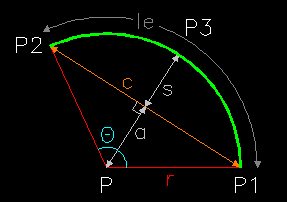
\includegraphics[width=0.5\textwidth]{figures/arcgeom.png}
	\captionof{figure}{Геометрия дуги окружности}
	\label{fig:arcgeom}
\end{figure}

Так как дуга окружности описывает часть этой окружности, то она и обладает всеми атрибутами данной окружности (см. рис. \ref{fig:arcgeom}). Среди них:

\begin{itemize}
	\item Радиус ($r$) --- радиус дуги такой же, как и у окружности;
	\item Центр ($P$) --- тот же, что и у окружности;
	\item Центральный угол ($\Theta$) --- в окружности равен $360^{\circ}$;
	\item Длина дуги ($le$) --- является частью периметра (длины) окружности.
\end{itemize}

Для дальнейшей работы с геометрией дуг примем, также, следующие специфичные атрибуты:

\begin{itemize}
	\item Начальная и конечная точка ($P1, P2$) --- это «вершины» дуги. Хотя иногда и целесообразно говорить о конкретных точках, не лежащих на концах дуги;
	\item Длина хорды ($c$) --- у дуг и окружностей можно провести бесконечное количество хорд, но для нас интерес представляет только хорда, проходящая через её вершины;
	\item Середина дуги ($P3$) --- точка, делящая дуги с данными вершинами на две, равные по длине, дуги;
	\item Апофема ($a$) --- это отрезок, вершинами которого являются середина дуги и её центр. Апофема перпендикулярна хорде;
	\item Высота дуги ($s$) --- это отрезок, проведённый из середины дуги перпендикулярно к хорде.
\end{itemize}

Кроме самой себя, дуга может, также, и описывать другие геометрические формы: круговой сегмент и сектор. Обе геометрические формы включают в себя все вышеперечисленные атрибуты, однако для выведения формулы параметра \textit{bulge} (выпуклости), потребуется рассмотрение только кругового сектора.

В документации AutoCAD \cite{Autodesk} выпуклостью называется тангенс четверти угла дуги между выбранной вершиной и следующей вершиной в списках вершин полилиний. Отрицательность параметра \textit{bulge} указывает на то, что дуга отрисовывается по часовой стрелке от выбранной вершины к следующей. Выпуклость, равная нулю --- прямой сегмент, выпуклость, равная единице --- половина окружности.

Проблема «расшифровки» атрибутов дуги для дальнейших манипуляций с ней заключается в том, что входными данными являются только координаты вершин и рассматриваемый параметр --- \textit{bulge}.

В самом деле, взяв арктангенс от параметра \textit{bulge} и умножив его на $4$, легко получить центральный угол, на который опирается рассматриваемая дуга. Результат получен в радианах. Для перевода значения в градусы, необходимо умножить это значение на $\pi$ и разделить на $180^{\circ}$.

Для вывода данной зависимости, рассмотрим дугу окружности (см. рис. \ref{fig:arcchord}).

\begin{figure}[H]
	\centering
	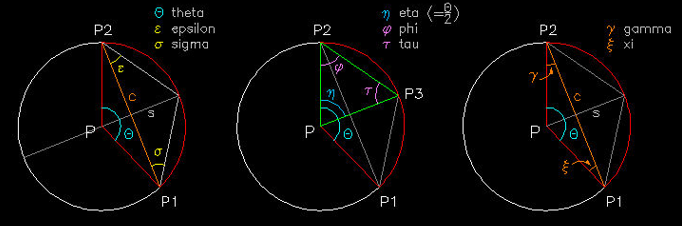
\includegraphics[width=1.0\textwidth]{figures/arcchord.png}
	\captionof{figure}{Дуга окружности с проведённой хордой и углами при ней}
	\label{fig:arcchord}
\end{figure}

Если провести к углу $\Theta$ биссектрису, то получится синий угол $\eta$. В итоге, мы получим равнобедренный треугольник (зеленый), в котором углы $\varphi$ и $\tau$ равны. Поскольку сумма углов в треугольнике всегда равна $180^{\circ}$ градусам, мы теперь знаем, что углы $\varphi$ и $\tau$ равны следующему (\ref{F:phi}):

\begin{equation}
	\varphi=\tau=\frac{(180^{\circ}-\frac{\Theta}{2})}{2}\Rightarrow\varphi=90^{\circ}-\frac{\Theta}{4}
	\label{F:phi}
\end{equation}

Теперь посмотрим на хорду $c$, проведённую от $P1$ до $P2$. Вместе с красными катетами угла $\Theta$ она тоже образует равнобедренный треугольник, а значит, $\gamma=\xi$. Угол при вершине треугольника $P-P1-P2$ --- это центральный угол $\Theta$, поэтому $\gamma$ и $\xi$ вычисляются следующим образом (\ref{F:gamma}):

\begin{equation}
	\gamma=\xi=\frac{180^{\circ}-\Theta}{2}\Rightarrow\gamma=90^{\circ}-\frac{\Theta}{2}
	\label{F:gamma}
\end{equation}

Таким образом, желтый угол $\varepsilon$ должен быть равняться разнице между фиолетовым углом $\varphi$ и оранжевым углом $\gamma$. Другими словами, $\varepsilon$ --- это четверть центрального угла $\Theta$ (\ref{F:epsilon}):

\begin{equation}
	\varepsilon=(90^{\circ}-\frac{\Theta}{4})-(90^{\circ}-\frac{\Theta}{2})\Rightarrow\varepsilon=\frac{\Theta}{2}-\frac{\Theta}{4}=\frac{\Theta}{4}
	\label{F:epsilon}
\end{equation}

Параметр \textit{bulge} (выпуклость) описывает, насколько дуга «выпирает» из вершин, то есть насколько велика высота дуги ($s$) (или расстояние от $P3$ до $P4$). Высота образует катет прямоугольного треугольника с углом, равным четверти центрального угла (см. желтый треугольник $P-P2-P3$ на рис. \ref{fig:epsilon}), и поскольку тангенс описывает отношение между катетами в прямоугольном треугольнике, легко описать геометрию с помощью этого одного угла (\ref{F:epsilon}):

\begin{equation}
	\frac{\sin(\varepsilon)}{\cos(\varepsilon)}=\tan(\varepsilon)
	\label{F:epsilon}
\end{equation}

\begin{figure}[H]
	\centering
	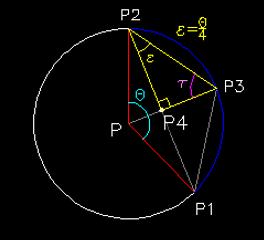
\includegraphics[width=0.5\textwidth]{figures/epsilon.png}
	\captionof{figure}{Связь угла $\varepsilon$ с центральным углом}
	\label{fig:epsilon}
\end{figure}

Мы, также, могли бы найти тангенс угла $\varepsilon$, просто разделив противолежащий катет на смежный катет --- что означает высоту дуги $s$, делённую на половину длины хорды $c$, --- но не зная $s$ и уже имея тангенс $\varepsilon$, полезнее найти $s$ (\ref{F:s}):

\begin{equation}
	s=\frac{c}{2}\cdot\tan(\varepsilon)
	\label{F:s}
\end{equation}

Примем

\begin{equation}
	\tan(\varepsilon)=bulge
	\label{F:tanepsilon}
\end{equation}

Тогда

\begin{equation}
	s=\frac{c}{2}\cdot bulge
	\label{F:sfinal}
\end{equation}

Таким образом, радиус дуги может быть найден следующим образом (\ref{F:r}):

\begin{equation}
	r=\frac{(\frac{c}{2})^2+s^2}{2s}
	\label{F:r}
\end{equation}

Знак той или иной выпуклости важен для определения дуги относительно вершин. Если выпуклость положительна, это означает, что дуга идёт против часовой стрелки от начальной вершины до конечной вершины. Если выпуклость отрицательна, это означает, что дуга идет, наоборот --- по часовой стрелке.

Поэтому все приведенные выше формулы должны касаться абсолютного значения выпуклости, а не фактического значения, иначе можно получить отрицательный радиус.

Итак, поняв, что $bulge = tan(\frac{\Theta}{4})$, в согласовании с документацией AutoCAD \cite{Autodesk} примем, что \textit{bulge} положителен, когда при передвижении от начальной точки дуги к конечной движение происходит против часовой стрелки.

Ясно, что когда $\Theta=0$, то и $bulge(\Theta)=0$. Для углов в $180^{\circ}$ условно принимается, что $bulge(\Theta)=\pm1$. В случае, когда $\Theta=90^{\circ}$, получим следующее (\ref{F:theta90}):

\begin{equation}
	bulge(90^{\circ})= \tan(\frac{90^{\circ}}{4})=\tan(\frac{\pi}{8})
	\label{F:theta90}
\end{equation}

Используя зависимость для тангенса половинного аргумента (\ref{F:tanhalfarg}):

\begin{equation}
	\tan(\frac{\alpha}{2})=\pm\frac{\sin(\frac{\alpha}{2})}{\cos(\frac{\alpha}{2})}=\pm\frac{2\sin^2(\frac{\alpha}{2})}{2\sin(\frac{\alpha}{2})\cos(\frac{\alpha}{2})}=\pm\frac{1-\cos(x)}{\sin(x)}
	\label{F:tanhalfarg}
\end{equation}

Для $\alpha=\frac{\pi}{8}$ получим (\ref{F:bulge90}):

\begin{equation}
	bulge(90^{\circ})=\tan(\frac{\pi}{8})=\pm\frac{1-\cos(\frac{\pi}{4})}{\sin(\frac{\pi}{4})}=\pm\frac{1-\frac{\sqrt2}{2}}{\frac{\sqrt2}{2}}=\pm\frac{1-\frac{1}{\sqrt2}}{\frac{1}{\sqrt2}}=\pm(\sqrt2-1)
	\label{F:bulge90}
\end{equation}



В результате, математические данные совпадают с документацией AutoCAD \cite{autocad2012dxf} и гласят, что

\begin{enumerate}
	\item $bulge = 0$ для отрезка прямой,
	\item $bulge = \pm1$ для дуги в $180^{\circ}$ (половина окружности),
	\item $bulge = \pm(\sqrt2-1) \approx0.41421...$ для четвертей окружностей, когда угол раствора дуги равен $90^{\circ}$.
\end{enumerate}

\section{Современное состояние проблемы конвертации данных в области САПР}
fvsfvs

\section{Постановка задачи}

\paragraph{Главные требования ко входному файлу}

Так как данная работа нацелена на создание ПО для обработки геометрической информации 2D-объектов специального типа, то конвертироваться из DXF-файлов должна не вся информация, содержащаяся в них. В первую очередь, заказчиком работы было определено, что на входе будет подаваться 2D-контур деталей типа <<Втулка>>, то есть тел вращения. Так как сконвертированная геометрия данных объектов в последующем предполагает разработку УП для токарных станков с ЧПУ, то геометрическая информация должна содержать определённый набор геометрических примитивов, с которым может работать система исполнительных органов станков с ЧПУ. Этот набор ограничивается тем, что исполнительные органы станков с ЧПУ способны перемещаться либо с помощью \textbf{линейной}, либо с помощью \textbf{круговой интерполяции}. Из этого следует, что для корректной работы САПР, для которых предназначаются разрабатываемые конвертеры, геометрия в DXF-файле на входе конвертеров должна состоять из, как минимум одного из представленных далее примитивов:

\begin{enumerate}
	\item линия (отрезок),
	\item полилиния,
	\item дуга,
	\item окружность.
\end{enumerate}

Остальные типы геометрии, реализуемой в формате DXF, такие как \textit{эллипс}, \textit{сплайн}, будут игнорироваться ПО.

На вход разрабатываемому конвертеру подаётся файл формата DXF. Формат DXF представляет собой совокупность данных с тегами всей информации, содержащейся в файле чертежа AutoCAD. Тегированные данные означают, что каждому элементу данных в файле предшествует целое число, называемое групповым кодом. Значение группового кода указывает, какой тип данных имеет следующий элемент. Это значение также указывает смысл элемента данных для данного типа объекта. Практически вся указанная пользователем информация в файле чертежа может быть представлена в формате DXF \cite{Autodesk}.
В DXF файлах, в зависимости от их содержания, существуют сущности, представляющие для нас интерес. Среди них следующие:

\begin{enumerate}
	\item LINE (Линия),
	\item LWPOLYLINE (Полилиния),
	\item ARC (Дуга),
	\item CIRCLE (Окружность),
	\item INSERT (Вставка).
\end{enumerate}

Как уже и было отмечено, существуют и другие примитивы (ELLIPSE, SPLINE и др.), однако, основываясь на конкретных целях заказчика по возможности применения выходных файлов для генерации УП, ПП проектируется только с указанными примитивами и сущностями DXF.

Рассмотрим каждую из сущностей подробнее.

\paragraph{LINE.} Рассмотрим тэги сущности \textit{Линия}, необходимые для её реального отображения (см. табл. \ref{tab:line}).


\begin{longtable}{|l|l|}
	\caption{Рассматриваемые групповые коды сущности LINE}
	\label{tab:line}
	\centering
	\tabularnewline
	\hline
	Групповой код & Описание\\
	\hline \endfirsthead
	\subcaption{Продолжение таблицы~\ref{tab:line}}
	\\ \endhead
	\subcaption{Продолжение на след. стр.}
	\endfoot
	%\hline
	\endlastfoot
	39	&	Толщина (необязательный; по умолч. = 0)\\ \hline
	10	&	Начальная точка (в с.к. объекта) DXF: значение X\\ \hline
	20, 30	&	DXF: Y и Z значения начальной точки (в с.к. объекта)\\ \hline
	11	&	Конечная точка (в с.к. объекта)	DXF: значение X\\ \hline
	21, 31	&	DXF: Y и Z значения конечной точки (в с.к. объекта)\\ \hline
\end{longtable}

\paragraph{LWPOLYLINE.} Рассмотрим тэги сущности \textit{Полилиния}, необходимые для её реального отображения (см. табл. \ref{tab:polyline}).

\begin{longtable}{|p{70pt}|p{370pt}|}
	\caption{Рассматриваемые групповые коды сущности POLYLINE}
	\label{tab:polyline}
	\centering
	\tabularnewline
	\hline
	Групповой код & Описание\\
	\hline \endfirsthead
	\subcaption{Продолжение таблицы~\ref{tab:polyline}}
	\\ \endhead
	\subcaption{Продолжение на след. стр.}
	\endfoot
	%\hline
	\endlastfoot
	70	&	«Флаг» полилинии (бит-закодировано); по умолч. = 0; 1 – закрыта\\ \hline
	39	&	Толщина (необязательный; по умолч. = 0)\\ \hline
	10	&	Координаты вершин (в с.к. объекта), множественные вхождения; по одному вхождению для каждой вершины DXF: значение X\\ \hline
	20	&	DXF: значение Y координат вершин (в с.к. объекта), множественные вхождения; по одному вхождению для каждой вершины\\ \hline
	42	&	\textit{Bulge}. Выпуклость (множественные вхождения - для каждой вершины), (необязательно; по умолч. =0)\\ \hline	
\end{longtable}

\paragraph{ARC.} Рассмотрим тэги сущности \textit{Дуга}, необходимые для её реального отображения (см. табл. \ref{tab:arc}).

\begin{longtable}{|p{70pt}|p{370pt}|}
	\caption{Рассматриваемые групповые коды сущности ARC}
	\label{tab:arc}
	\centering
	\tabularnewline
	\hline
	Групповой код & Описание\\
	\hline \endfirsthead
	\subcaption{Продолжение таблицы~\ref{tab:arc}}
	\\ \endhead
	\subcaption{Продолжение на след. стр.}
	\endfoot
	%\hline
	\endlastfoot
	39	&	Толщина (необязательный; по умолч. = 0)\\ \hline	
	10	&	Центр дуги (в с.к. объекта)
	DXF: значение X\\ \hline	
	20, 30	&	DXF: Y и Z значения центра дуги (в с.к. объекта)\\ \hline	
	40	&	Радиус\\ \hline	
	50	&	Начальный угол\\ \hline	
	51	&	Конечный угол\\ \hline	
\end{longtable}

\paragraph{CIRCLE.} Рассмотрим тэги сущности \textit{Окружность}, необходимые для её реального отображения (см. табл. \ref{tab:circle}).

\begin{longtable}{|p{70pt}|p{370pt}|}
	\caption{Рассматриваемые групповые коды сущности CIRCLE}
	\label{tab:circle}
	\centering
	\tabularnewline
	\hline
	Групповой код & Описание\\
	\hline \endfirsthead
	\subcaption{Продолжение таблицы~\ref{tab:circle}}
	\\ \endhead
	\subcaption{Продолжение на след. стр.}
	\endfoot
	%\hline
	\endlastfoot
	39	&	Толщина (необязательный; по умолч. = 0)\\ \hline	
	10	&	Центр дуги (в с.к. объекта)
	DXF: значение X\\ \hline	
	20, 30	&	DXF: Y и Z значения центра дуги (в с.к. объекта)\\ \hline	
	40	&	Радиус\\ \hline	
	50	&	Начальный угол\\ \hline	
	51	&	Конечный угол\\ \hline	
\end{longtable}

\paragraph{INSERT.} Данная сущность представляет собой вставку блоков с геометрией. Её необходимо рассматривать, так как геометрия может быть вложенной и, таким образом, не видна обзорщиком сущностей, так как вложена. У этой сущности поиск информации по тэгам в программе не потребуются.


\section{Выводы по главе \ref{cha:aktuell}}
fsfgsdfs
